\chapter{Proposed Implementation}
\label{ch:proposed-implementation}

Once all the objectives and requirements to be achieved have been described,
the different systems and techniques existing to achieve them have been studied,
and their contributions and shortcomings have been evaluated, we will describe
the proposed solution both in terms of design and possible implementation

\section{Structure}
The system is divided into components so that each component works on its input
and produces its output. In this way, a parser is achieved that behaves like
an API where each element can be called individually. \cref{fig:shex-lite-sema}
shows the different components of this analyser.

\begin{figure}
    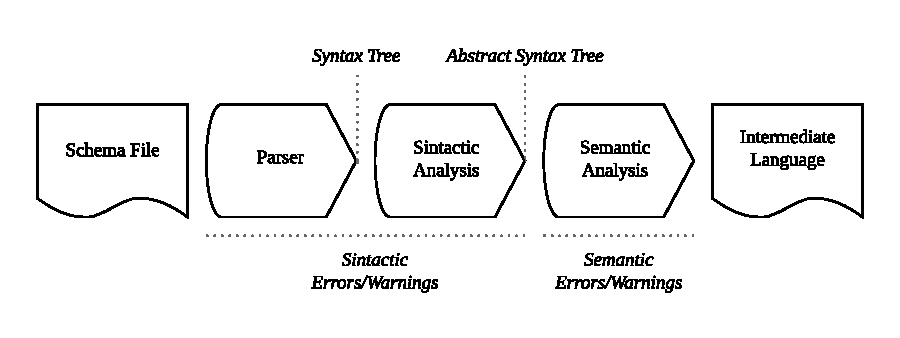
\includegraphics[width=\textwidth]{images/sin-sem-structure.pdf}
    \centering
    \caption[Syntactic and Semantic Analyser structure]{Syntactic and Semantic Analyser structure.}
    \label{fig:shex-lite-sema}
\end{figure}

\subsection{Parser}
We define the parsing stage as the process that begins when we receive the source code that makes up
the schema until the moment we produce a syntax tree. Therefore it includes the conversion to tokens
by the lexer, the grouping of tokens in rules and later in a syntax tree by the parser.

The general idea of this stage is that you take the source code as input and build a syntactic tree with all
the possible information from the source code. This implies that the syntactic tree is not only made up of
abstract grammar, but also of separators, braces and keywords. \cref{fig:shex-lite-st} shows an example
of the first 20 nodes generated by the parser. There we can see this composition of separators, keywords, braces
and content.

\begin{figure}
    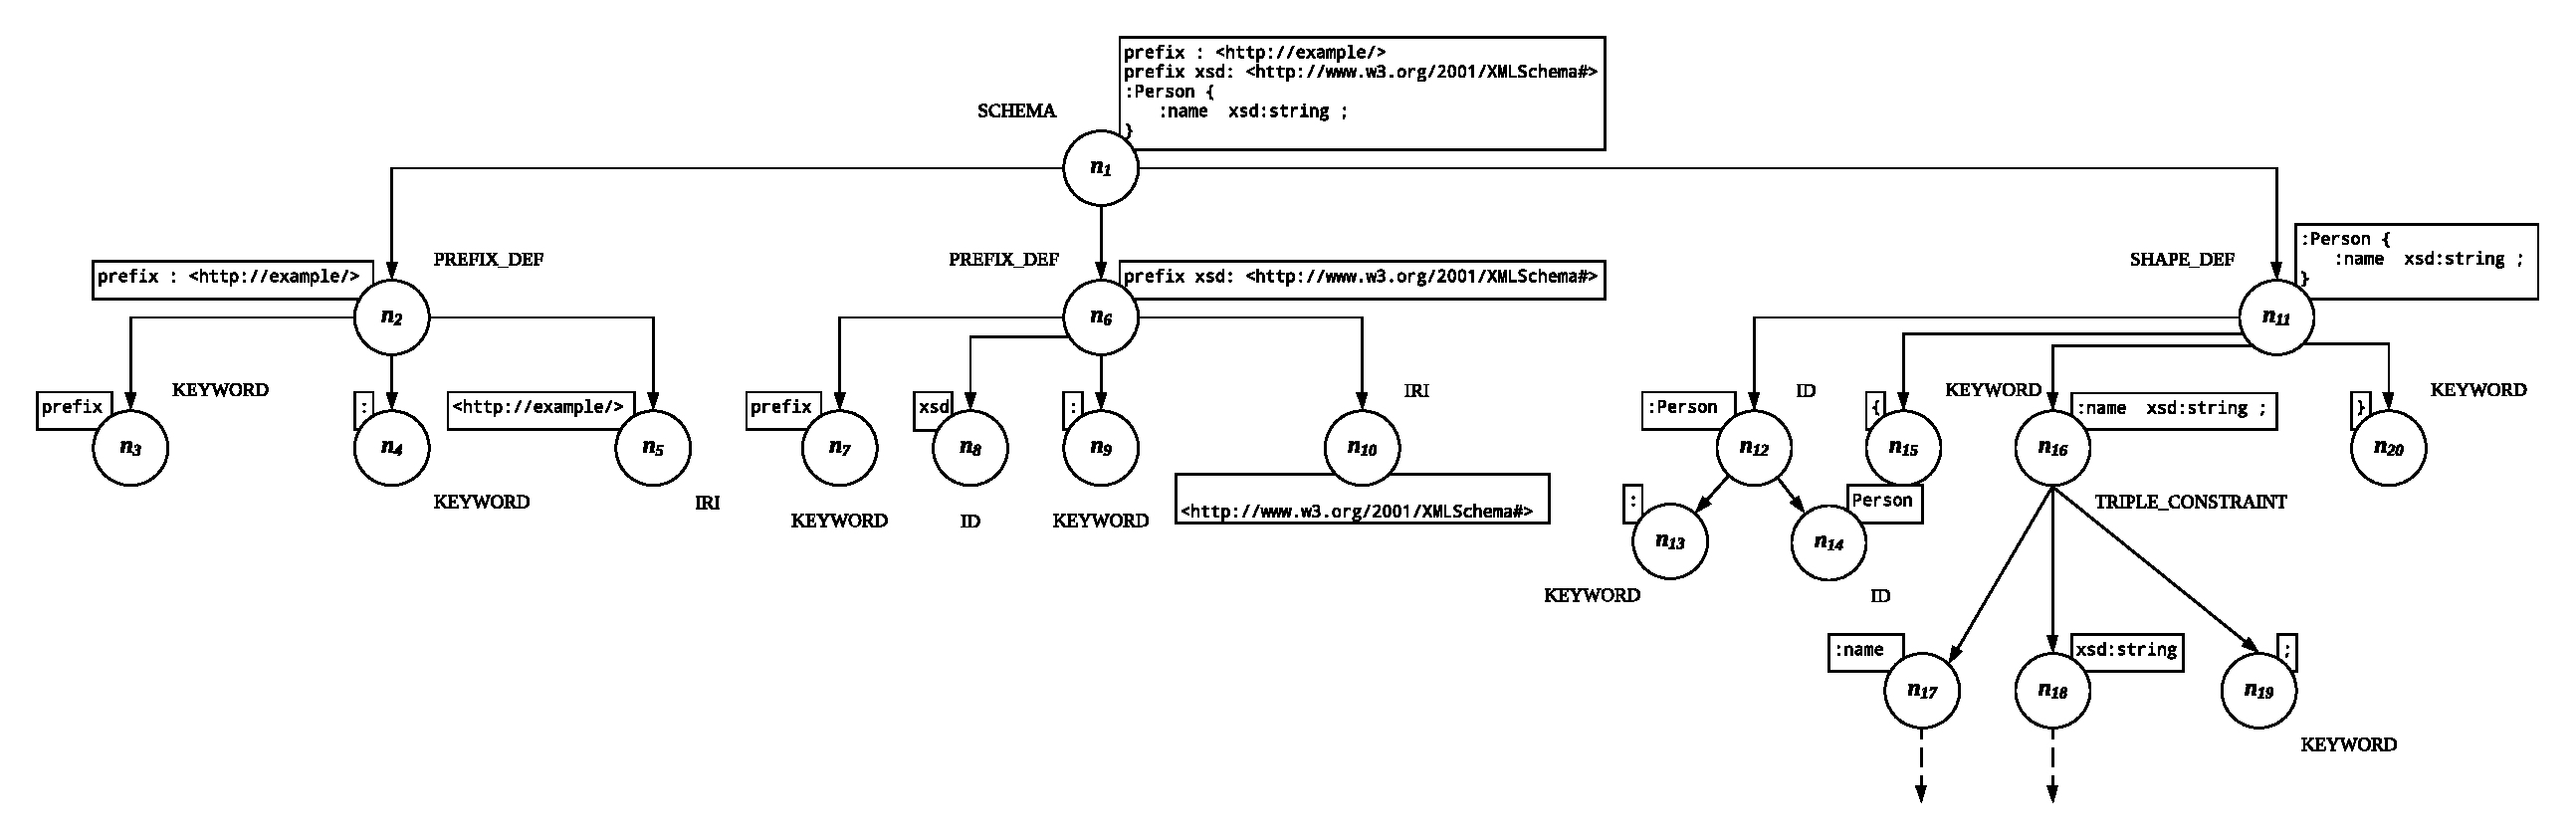
\includegraphics[width=\textwidth]{images/shex-lite-syntax-tree.pdf}
    \centering
    \caption[Syntax Tree twenty first nodes produced by the parser]{Syntax Tree twenty first nodes produced by the parser.}
    \label{fig:shex-lite-st}
\end{figure}

Once we have the complete syntactic tree generated, we can go through it to carry out syntactic analysis on the different elements.
For example, in the tree in \cref{fig:shex-lite-st} we could implement a validator that in the event that the last triple constraint
of a shape definition \textit{(node 16)} did not have the semicolon termination keyword \textit{(node 19)}, it would generate a
warning message to the user.

\subsection{Syntactic Analyser}
The Syntactic analyser is in charge of traversing the syntactic tree in order to search for possible patterns that the user has to
be informed about. If none were found it would be understood that the syntactic tree is well formed and it will transform the Syntax Tree
\cref{fig:shex-lite-st} into an Abstract Syntax Tree \cref{fig:shex-lite-sema-anal} \textit{(without the green and red relations)}.

For this, each node within our syntactic tree is aware of the context in which it is. Therefore, it is possible to access contextual
information of a given node. For instance, we can access to to a prefix definition (\cref{fig:shex-lite-st} $n_2$)) contextual
information to check if it contains a label. It does not contain one. Or access the information of (node $n_5$) to get the
node that defines its iri. Would be (node $n_5$). With questions like these, the syntactic tree can be analysed for patterns that
represent warnings or errors.

\subsection{Semantic Analyser}
The semantic analyser is responsible of building all the possible relations between the AST nodes, analyse and check that
all those relations that must exist indeed exist. For this porpoise as just seen we reduce our Syntax Tree to an
Abstract Syntax Tree. \cref{fig:shex-lite-sema-anal} Shows the resulting AST after the corresponding analysis and
transformations, we call this graph the \textit{Intermediate Language}.

\begin{figure}
    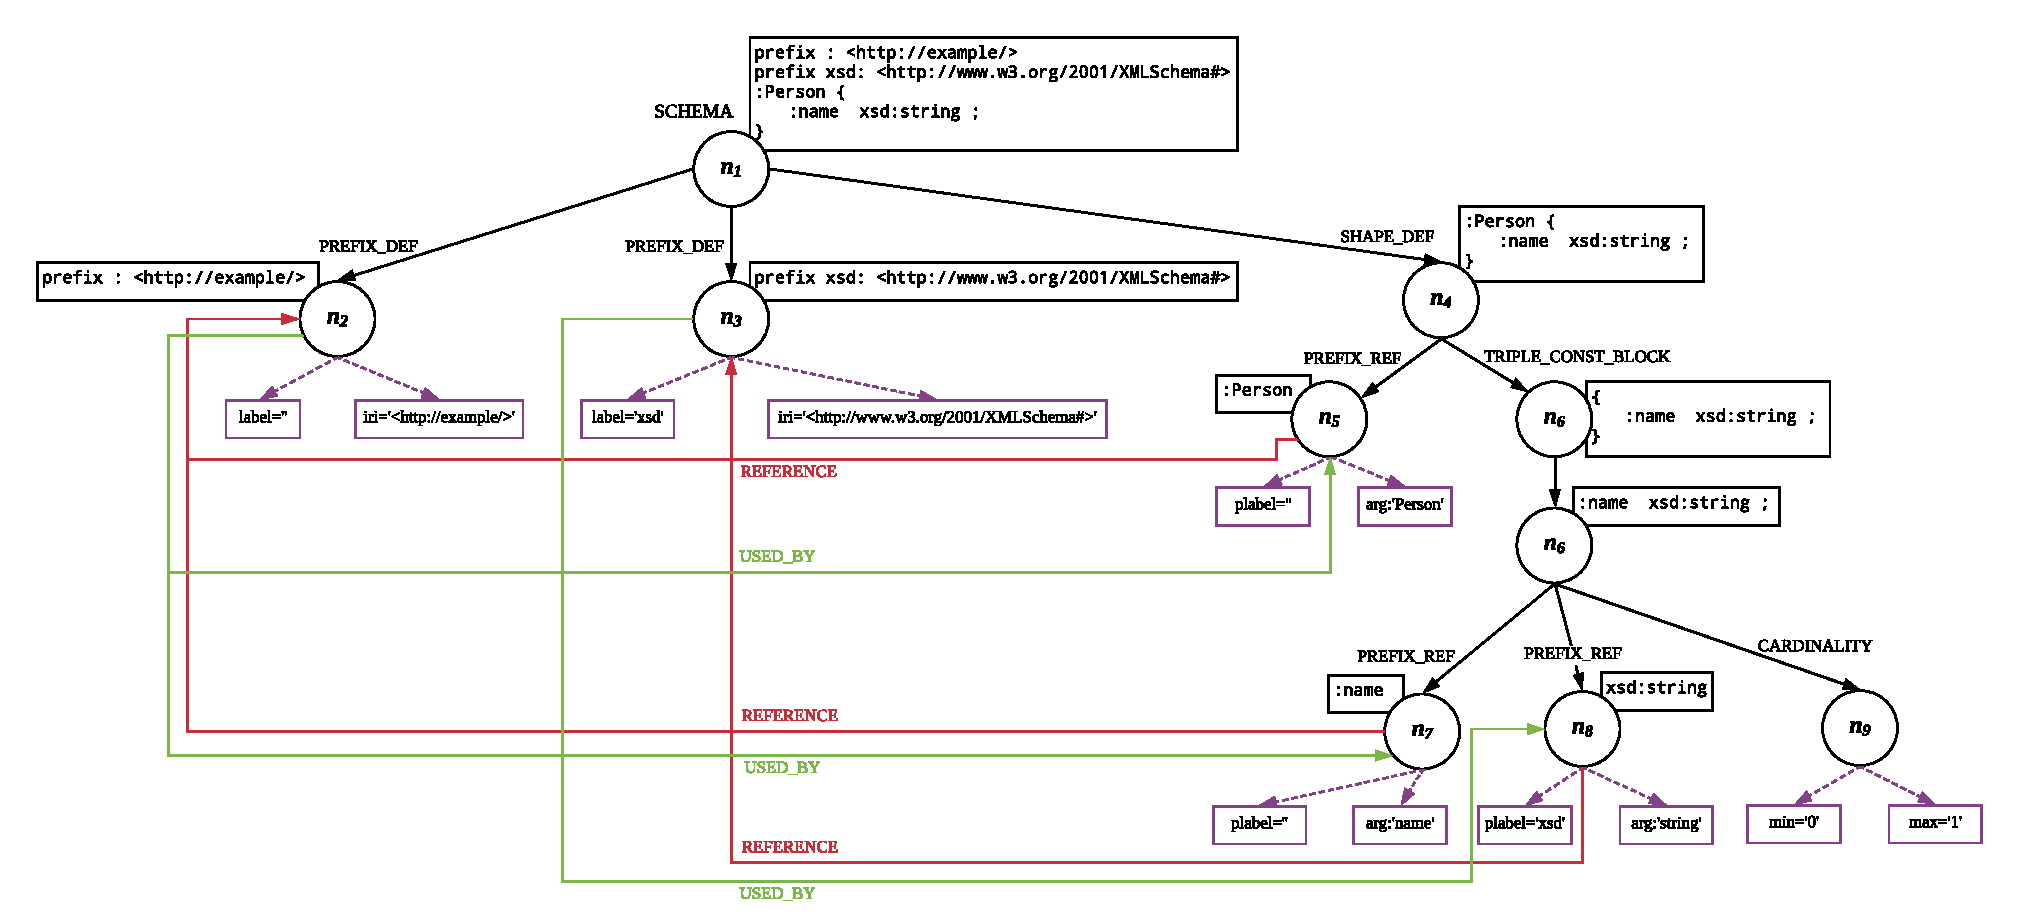
\includegraphics[width=\textwidth]{images/shex-lite-sema-anal.pdf}
    \centering
    \caption[Abstract Syntax Tree produced after validation and transformations]{Abstract Syntax Tree produced after validation and
    transformations.}
    \label{fig:shex-lite-sema-anal}
\end{figure}

Once we have the representation modelled and this representation is capable of expressing all the assumptions of our language,
we can begin to apply validators on our structure. For example if we wanted to find broken references we could go to the nodes
that are a reference to definitions like nodes $n_{\:5,\:7\:and\:8}$ and check that there is indeed a valid reference for each of them.

Furthermore, we can even analyse how many times a definition is used by a reference so that we can launch messages warning the end user
in some cases, such as when a prefix is not used.

\section{Implementation}\label{sec:anal-implementation}
As proof of concept of the previous proposal we offer an implementation of the three components, the parser, the Syntactic analyser
and the semantic parser. The implementation is defined in the same way as the structure, in three parts. We will now explore each
of those parts and their responsibilities separately.

\subsection{Parser}
As previously discussed, the function of the parser is to extract a syntactic tree from the diagrams that we can analyse.
For this purpose we decided to use the Antlr tool \cite{parr1995antlr}. This tool is capable of generating Syntactic analysers
from grammars defined in its own syntax. However, this tool is focused on completely processing the syntax tree and producing
only the abstract syntax tree. Therefore we had to use a modification of the original ShEx micro Compact Syntax syntax so that
Antlr would produce a tree with all the syntactic content. This also does offer the flexibility that in the future if we want to
implement any additional syntactic validation we simply have to do it on the tree that the parser generates for
us and not on the Antlr code.

\subsection{Syntactic Analyser}
The Syntactic analyser has the responsibility to validate that the parser produced syntax tree is correct and to build the abstract syntax
tree as well. To do this, it uses the same mechanism. Through the visitor pattern we go through our syntax tree. Each implementation
of this visitor has a purpose, for example an implementation can go through a few specific nodes to validate them syntactically
while another can go through them in order to build the AST. \cref{fig:checker-example} shows an example of how a Syntactic check is
implemented.

\begin{figure}
    \begin{lstlisting}[language=Java,numbers=left,basicstyle=\ttfamily\scriptsize]
override def visitConstraint_triple_expr(...) {
  if(/*No trailing semicolon*/)
    //Warn user about this bad practice
}
    \end{lstlisting}
    \caption[Checker implementation for missing semicolons warning generation]{Checker implementation for missing semicolons warning generation.}
    \label{fig:checker-example}
\end{figure}

The AST construction stage is very delicate since for each generated node we have to include as much context information as possible
so that when an error is detected in the tree we can identify not only the cause but also the position, the origin, the rest of the
affected nodes and therefore offer a content-rich error message. Regarding our implementation, for each node we save the following
context information:
\begin{itemize}
    \item \textbf{Source file path.} It represents the path to the source file where the node was generated.
    \item \textbf{Line.} The line in the source file where the node was generated.
    \item \textbf{Column.} The column in the source file where the node was generated.
    \item \textbf{Token interval.} The interval \textit{(start, end position)} of tokens from the source file that generated the node.
    \item \textbf{Content.} The content of the node as plain text. \cref{fig:shex-lite-sema-anal} is very representative of this. 
    \item \textbf{Parent node.} A pointer to the parent node.
    \item \textbf{Children nodes.} A list of pointers to all the children nodes.
\end{itemize}

\cref{fig:shex-lite-node-info} represents this information inside each node. Our default implementation only looks for the
following extra syntactic pattern to the other implementations seen in \cref{ch:current-analysers-analysis}: shape expressions whose last
triple constraint does not contain the semicolon ending character. In case we find this pattern, we inform the event manager
that a notice has been found that must be passed on to the user, \cref{fig:sin-err-example}.

\begin{figure}
    \begin{lstlisting}[numbers=left,basicstyle=\ttfamily\scriptsize]
warning[W005]: missing semicolon
--> shape_with_warning_cause_semicolon.shexl:8:23
    |
8   | :knows      @:User *
    |                      ^ semicolons are not compulsory in the last triple constraint,
                             but its usage its encouraged as otherwise your code wont be
                             following shape expressions specification.
    \end{lstlisting}
    \caption[Syntactic warning produced by the proposed Syntactic analyser]{Syntactic warning produced by the proposed Syntactic analyser.}
    \label{fig:sin-err-example}
\end{figure}

\begin{figure}
    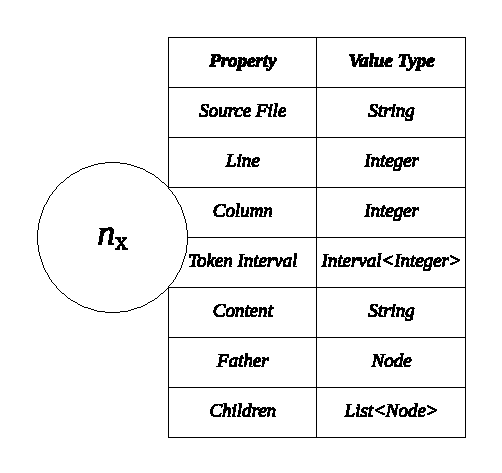
\includegraphics[scale=0.7]{images/shex-lite-node-table.pdf}
    \centering
    \caption[Common information stored at any AST node]{Common information stored at any AST node.}
    \label{fig:shex-lite-node-info}
\end{figure}

\subsection{Semantic Analyser}
Recall that the semantic analyser takes the generated AST, runs it in search of errors and transforms it in such a way that
it emits a graph that corresponds to the intermediate language. We can separate semantic analysis into two phases, a first
one in which we transform our syntactic tree, adding possible relationships. And a second phase in which we analyse existing
and created relationships.

\subsubsection{Tree transformations}
In the case of our syntax the semantic relations that we find is the linking of a reference to its definition and the opposite
direction to indicate that a definition is being referenced by a node. The transformations are listed bellow:

\begin{itemize}
    \item \textbf{Linking prefix definition with prefix references.} Prefix references occurs when a node describes itself as
    the composition of a prefix and an argument. The idea is that the prefix substitute the IRI, but must be linked as any
    prefix reference needs to point to an existing definition.
    \item \textbf{Linking base definition with base references.} Some nodes are defined as relative IRIs to the base definition
    and therefore need to be linking to them in order to be able to get that base IRI.
    \item \textbf{Linking shape definition with a shape reference.} Shape definitions can be used at the \texttt{start} definition
    to point the default shape or as type constraints in the triple constraints. At any of those points shape references must
    exist within the scope of an schema.
\end{itemize}

\subsubsection{Tree relations analysis}
For this purpose, the semantic analyser defines the visitor pattern on the nodes of the abstract syntax tree so that each of the different
analysis is done with a tree visiting implementation.

\section{Tests}
Different types of tests were used to validate the implementation. Of course, unitary, integration, regression.
However, the most important in here are the dynamic test cases. In this way it was possible to test the
system just by describing test cases using files. These files represent the input of the test system. And according
to the file name, it is automatically classified as positive or negative test. A battery of tests defined by the
people who carried out the ShEx specification have been used to tests the system. In our case with 45 different test
scenarios. In addition, to ensure compatibility with all platforms, continuous integration with GitHub has been made
over Windows, Linux and Mac OS. A coverage of the 70\% of the code is achieved.
See \cref{ch:github} to see the CI configuration.

\section{Syntactic and Semantic Error and Warnings Detected}
With the solution proposed in the previous section, our system is capable of detecting and reporting multiple syntactic
and / or semantic errors. In this section we will analyse the rules that generate each type of event and the different
error messages produced for each one of them.

\subsection{Not trailing semicolon at last triple constraint}
To detect when the semicolon is missing in the last triple constraint of a shape definition, the rule used is very simple.
Find the last node in the triple constraints list of a shape definition. And once this node is found, it is searched whether or
not it contains the final token character that corresponds to a semicolon. If it does not have it, a warning message is generated,
indicating the position through file, line, column and context, which is sent to the compilation event manager, which in turn gives
the corresponding format to print the message. \cref{fig:sin-err-example} shows an example of this message.

\subsection{Prefix not defined}
These types of events happen when we use a reference to a prefix and this has not been defined in the scope of the schema.
In the event that this happens we have an error that we cannot recover from since we cannot associate the reference to anything.

In order to detect this assumption, all the prefix definitions have to be traversed previously and for each one of them,
a record will have to be created in a symbol table where it is indexed by the label and a reference to the definition node
is added. All types of type reference to prefix can then be accessed and for each one it is verified that the label exists
in the symbol table and then a pointer to the corresponding definition node is added to the reference node. If, on the other hand,
a definition cannot be found in the symbol table, then an error message like \cref{fig:err-non-def-pref} is created.

For example in the \cref{fig:shex-lite-sema-anal} the red lines would be the transformations done to the original AST to
add the pointers to the reference nodes that point to the definition nodes.

\begin{figure}
    \begin{lstlisting}[numbers=left,basicstyle=\ttfamily\scriptsize]
error[E007]: prefix not defined
--> shape_with_error_cause_pref_not_defined.shex:17:3
    |
17  | non_existing:label  xsd:string  +;
    | ^ the prefix `non_existing` has not been defined
    \end{lstlisting}
    \caption[Semantic error produced by an undefined prefix]{Semantic error produced by an undefined prefix.}
    \label{fig:err-non-def-pref}
\end{figure}

\subsection{Shape not defined}
In the same way as the previous case, an undefined shape error occurs in the case that there is a reference to a shape
expression that is not defined in the scope of the schema.

For this, all the definitions of shape expressions of our schema must have been previously identified and indexed in
a symbol table where the key is the name and the value a reference to the node of the definition. Once the definitions
of shape expressions have been identified, we only have to go through those nodes of type reference to shape expression
and look for a definition of a shape expression with the corresponding label within the scope of the prefix specified
in the reference. If it exists, a reference is added to the type reference to shape that points to the corresponding
definition. Otherwise, an error message like \cref{fig:err-non-def-shape} is generated.

\begin{figure}
    \begin{lstlisting}[numbers=left,basicstyle=\ttfamily\scriptsize]
error[E008]: shape not defined
--> shape_with_error_cause_shape_not_defined.shex:16:13
    |
16  | @existing_prefix:Not_Existing_Shape
    |                  ^ the shape `Not_Existing_Shape` has not been defined
                         in the scope of the prefix `existing_prefix`
    \end{lstlisting}
    \caption[Semantic error produced by an undefined shape]{Semantic error produced by an undefined shape.}
    \label{fig:err-non-def-shape}
\end{figure}

\subsection{Prefix overridden}
We say that a prefix is overwritten when we come across a second prefix definition that tries to assign any
value to a prefix that had already been defined previously.

For this, during the identification of prefixes, every time we find a prefix type node we try to add a record
to our symbol table. In this entry, the key will be the prefix label. If there is already an entry in the symbol
table with the same tag, then we would be facing a prefix override. So instead of taking the action we would
throw an error message like \cref{fig:err-override-prefix}.

\begin{figure}
    \begin{lstlisting}[numbers=left,basicstyle=\ttfamily\scriptsize]
error[E003]: attempt to override an already defined prefix
--> shape_with_error_cause_prefix_override.shex:15:0
    |
15  | PREFIX foaf: <hppt://another/value>
    | ^ this prefix definition overrides the previous one (9:0) with
        value <http://xmlns.com/foaf/0.1/>
    \end{lstlisting}
    \caption[Semantic error produced by a prefix override]{Semantic error produced by a prefix override.}
    \label{fig:err-override-prefix}
\end{figure}

\subsection{Shape overridden}
The case of a shape expression overwriting is slightly less trivial in that a shape is identified as the
union of an existing prefix and a unique identifier within the ambit of that prefix. Therefore, the way
of acting will be (assuming that the prefix exists, if it would not be another error) check if a shape
definition with the same identifier already exists within the scope of the indicated prefix. If it exists
we will throw an error like the one from \cref{fig:err-override-shape}. If not, we will add a record to the
indicated prefix scope with the corresponding information from the shape definition.

\begin{figure}
    \begin{lstlisting}[numbers=left,basicstyle=\ttfamily\scriptsize]
error[E004]: attempt to override an already defined shape
--> shape_with_error_cause_shape_override.shex:40:0
    |
40  | :Q3559 {
    |  ^ this shape definition overrides the previous one (17:0)
41  |   schema:name xsd:string ;
42  | }
    \end{lstlisting}
    \caption[Semantic error produced by a shape override]{Semantic error produced by a shape override.}
    \label{fig:err-override-shape}
\end{figure}

\subsection{Unused prefix definition}
One of the small optimizations that our semantic solution includes is the early detection of resources
not defined as prefixes. In addition, it is a use case of semantic statistics generated by our proposed
solution. In this specific case, what is checked is the number of resources that use a definition. For this,
the symbol table is consulted since this is the one that stores this information. It corresponds to the
relationships in green in \cref{fig:shex-lite-sema-anal}.

In the event that a prefix definition has zero resources that use it, the prefix is not used and therefore
it can be removed without problem since it only takes up space. To warn the user of this, a warning like \cref{fig:warn-pref-not-used}
is generated

\begin{figure}
    \begin{lstlisting}[numbers=left,basicstyle=\ttfamily\scriptsize]
warning[W001]: prefix definition not used
--> shape_with_warning_cause_prefix_never_used.shex:8:12
    |
8   | PREFIX owl: <http://www.w3.org/2002/07/owl#>
    |        ^ the prefix `owl` definition is never used
    \end{lstlisting}
    \caption[Semantic warning produced by a prefix never used]{Semantic warning produced by a prefix never used.}
    \label{fig:warn-pref-not-used}
\end{figure}

\subsection{Base set but not used}
Another case in which the early detection of unused resources is used is with the definition of the base.
If for some reason a user assigns a value to the base but never uses it, a warning like \cref{fig:warn-base-not-used}
is generated.

\begin{figure}
\begin{lstlisting}[numbers=left,basicstyle=\ttfamily\scriptsize]
warning[W002]: base has been set but not used
--> shape_with_warning_cause_base_set_but_never_used.shex:17:5
    |
17  | BASE <http://a/base/not/used/value>
    |      ^ the base `<http://a/base/not/used/value>` definition is
             set but not used
    \end{lstlisting}
    \caption[Semantic warning produced by a base set but never used]{Semantic warning produced by a base set but never used.}
    \label{fig:warn-base-not-used}
\end{figure}